% Created by tikzDevice version 0.12.3.1 on 2021-12-06 11:34:02
% !TEX encoding = UTF-8 Unicode
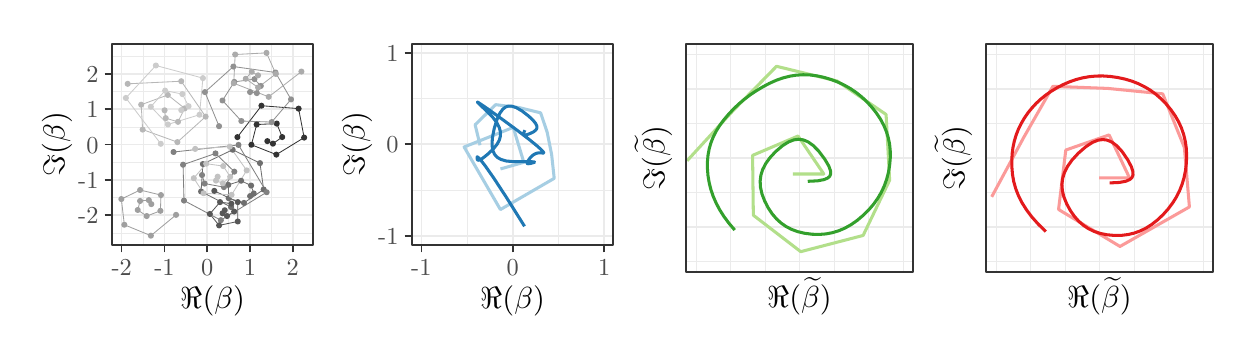
\begin{tikzpicture}[x=1pt,y=1pt]
\definecolor{fillColor}{RGB}{255,255,255}
\begin{scope}
\definecolor{drawColor}{RGB}{255,255,255}
\definecolor{fillColor}{RGB}{255,255,255}

\path[draw=drawColor,line width= 0.6pt,line join=round,line cap=round,fill=fillColor] ( -0.00,  5.56) rectangle (108.41,114.41);
\end{scope}
\begin{scope}
\definecolor{fillColor}{RGB}{255,255,255}

\path[fill=fillColor] ( 30.25, 36.25) rectangle (102.91,108.91);
\definecolor{drawColor}{gray}{0.92}

\path[draw=drawColor,line width= 0.3pt,line join=round] ( 30.25, 40.54) --
	(102.91, 40.54);

\path[draw=drawColor,line width= 0.3pt,line join=round] ( 30.25, 53.30) --
	(102.91, 53.30);

\path[draw=drawColor,line width= 0.3pt,line join=round] ( 30.25, 66.06) --
	(102.91, 66.06);

\path[draw=drawColor,line width= 0.3pt,line join=round] ( 30.25, 78.83) --
	(102.91, 78.83);

\path[draw=drawColor,line width= 0.3pt,line join=round] ( 30.25, 91.59) --
	(102.91, 91.59);

\path[draw=drawColor,line width= 0.3pt,line join=round] ( 30.25,104.36) --
	(102.91,104.36);

\path[draw=drawColor,line width= 0.3pt,line join=round] ( 41.39, 36.25) --
	( 41.39,108.91);

\path[draw=drawColor,line width= 0.3pt,line join=round] ( 56.84, 36.25) --
	( 56.84,108.91);

\path[draw=drawColor,line width= 0.3pt,line join=round] ( 72.29, 36.25) --
	( 72.29,108.91);

\path[draw=drawColor,line width= 0.3pt,line join=round] ( 87.74, 36.25) --
	( 87.74,108.91);

\path[draw=drawColor,line width= 0.6pt,line join=round] ( 30.25, 46.92) --
	(102.91, 46.92);

\path[draw=drawColor,line width= 0.6pt,line join=round] ( 30.25, 59.68) --
	(102.91, 59.68);

\path[draw=drawColor,line width= 0.6pt,line join=round] ( 30.25, 72.45) --
	(102.91, 72.45);

\path[draw=drawColor,line width= 0.6pt,line join=round] ( 30.25, 85.21) --
	(102.91, 85.21);

\path[draw=drawColor,line width= 0.6pt,line join=round] ( 30.25, 97.97) --
	(102.91, 97.97);

\path[draw=drawColor,line width= 0.6pt,line join=round] ( 33.66, 36.25) --
	( 33.66,108.91);

\path[draw=drawColor,line width= 0.6pt,line join=round] ( 49.11, 36.25) --
	( 49.11,108.91);

\path[draw=drawColor,line width= 0.6pt,line join=round] ( 64.56, 36.25) --
	( 64.56,108.91);

\path[draw=drawColor,line width= 0.6pt,line join=round] ( 80.02, 36.25) --
	( 80.02,108.91);

\path[draw=drawColor,line width= 0.6pt,line join=round] ( 95.47, 36.25) --
	( 95.47,108.91);
\definecolor{drawColor}{gray}{0.20}

\path[draw=drawColor,line width= 0.3pt,line join=round] ( 86.31, 73.72) --
	( 88.32, 72.80) --
	( 91.67, 75.18) --
	( 89.71, 80.05) --
	( 82.44, 79.71) --
	( 80.56, 72.40) --
	( 89.56, 68.84) --
	( 99.60, 74.99) --
	( 97.60, 85.46) --
	( 84.18, 86.51) --
	( 75.49, 75.16);
\definecolor{drawColor}{gray}{0.34}

\path[draw=drawColor,line width= 0.3pt,line join=round] ( 70.92, 48.74) --
	( 70.12, 47.64) --
	( 71.74, 46.64) --
	( 74.31, 48.27) --
	( 73.30, 51.12) --
	( 69.22, 51.68) --
	( 65.52, 47.39) --
	( 68.87, 43.27) --
	( 75.61, 44.68) --
	( 75.63, 51.68) --
	( 67.14, 55.74);
\definecolor{drawColor}{gray}{0.43}

\path[draw=drawColor,line width= 0.3pt,line join=round] ( 80.08, 53.85) --
	( 81.40, 54.80) --
	( 80.44, 57.66) --
	( 76.82, 59.39) --
	( 72.19, 57.90) --
	( 72.33, 53.09) --
	( 77.84, 51.39) --
	( 84.97, 56.24) --
	( 83.64, 65.76) --
	( 73.76, 70.60) --
	( 63.01, 65.44) --
	( 62.36, 55.51) --
	( 73.18, 49.89);
\definecolor{drawColor}{RGB}{129,129,129}

\path[draw=drawColor,line width= 0.3pt,line join=round] ( 62.71, 61.46) --
	( 63.64, 58.38) --
	( 70.61, 57.09) --
	( 74.37, 62.69) --
	( 67.57, 69.27) --
	( 55.85, 65.19) --
	( 56.19, 52.24) --
	( 69.50, 45.15) --
	( 86.05, 55.25) --
	( 75.88, 72.34) --
	( 52.41, 69.78);
\definecolor{drawColor}{gray}{0.57}

\path[draw=drawColor,line width= 0.3pt,line join=round] ( 80.06, 91.44) --
	( 82.50, 91.06) --
	( 83.94, 93.65) --
	( 81.65, 96.11) --
	( 74.36, 95.12) --
	( 70.10, 88.40) --
	( 76.91, 80.98) --
	( 87.88, 80.60) --
	( 94.86, 88.79) --
	( 89.24, 98.52) --
	( 74.03,100.66) --
	( 63.75, 91.43) --
	( 68.85, 79.11);
\definecolor{drawColor}{RGB}{159,159,159}

\path[draw=drawColor,line width= 0.3pt,line join=round] ( 44.37, 50.96) --
	( 43.48, 52.39) --
	( 40.32, 52.09) --
	( 39.47, 48.83) --
	( 42.71, 46.64) --
	( 47.67, 48.53) --
	( 47.86, 54.22) --
	( 40.33, 56.05) --
	( 33.55, 52.78) --
	( 34.63, 43.49) --
	( 44.22, 39.55) --
	( 53.32, 47.07);
\definecolor{drawColor}{gray}{0.67}

\path[draw=drawColor,line width= 0.3pt,line join=round] ( 82.94, 97.48) --
	( 80.67, 98.78) --
	( 78.50, 96.24) --
	( 82.96, 93.09) --
	( 89.37, 98.00) --
	( 86.00,105.60) --
	( 74.68,105.01) --
	( 74.16, 94.63) --
	( 86.79, 89.72) --
	( 98.62, 98.85);
\definecolor{drawColor}{RGB}{183,183,183}

\path[draw=drawColor,line width= 0.3pt,line join=round] ( 49.17, 84.86) --
	( 49.59, 82.00) --
	( 54.02, 80.69) --
	( 56.44, 85.54) --
	( 50.33, 90.39) --
	( 40.72, 86.87) --
	( 41.24, 77.89) --
	( 53.80, 73.36) --
	( 64.01, 82.57) --
	( 55.19, 95.36) --
	( 35.84, 94.42);
\definecolor{drawColor}{gray}{0.76}

\path[draw=drawColor,line width= 0.3pt,line join=round] ( 68.35, 60.87) --
	( 67.76, 59.44) --
	( 70.21, 58.48) --
	( 72.88, 60.84) --
	( 70.36, 64.70) --
	( 64.21, 65.56) --
	( 59.72, 60.32) --
	( 63.28, 54.87) --
	( 73.38, 54.30) --
	( 78.85, 63.13) --
	( 72.74, 71.73) --
	( 60.23, 70.90);
\definecolor{drawColor}{gray}{0.80}

\path[draw=drawColor,line width= 0.3pt,line join=round] ( 55.21, 84.92) --
	( 57.83, 86.34) --
	( 55.60, 90.72) --
	( 49.37, 91.97) --
	( 44.20, 86.14) --
	( 50.37, 79.75) --
	( 61.79, 83.25) --
	( 63.02, 96.48) --
	( 46.03,101.04) --
	( 35.18, 89.31) --
	( 47.79, 72.75);
\definecolor{drawColor}{gray}{0.20}
\definecolor{fillColor}{gray}{0.20}

\path[draw=drawColor,line width= 0.4pt,line join=round,line cap=round,fill=fillColor] ( 86.31, 73.72) circle (  0.89);

\path[draw=drawColor,line width= 0.4pt,line join=round,line cap=round,fill=fillColor] ( 88.32, 72.80) circle (  0.89);

\path[draw=drawColor,line width= 0.4pt,line join=round,line cap=round,fill=fillColor] ( 91.67, 75.18) circle (  0.89);

\path[draw=drawColor,line width= 0.4pt,line join=round,line cap=round,fill=fillColor] ( 89.71, 80.05) circle (  0.89);

\path[draw=drawColor,line width= 0.4pt,line join=round,line cap=round,fill=fillColor] ( 82.44, 79.71) circle (  0.89);

\path[draw=drawColor,line width= 0.4pt,line join=round,line cap=round,fill=fillColor] ( 80.56, 72.40) circle (  0.89);

\path[draw=drawColor,line width= 0.4pt,line join=round,line cap=round,fill=fillColor] ( 89.56, 68.84) circle (  0.89);

\path[draw=drawColor,line width= 0.4pt,line join=round,line cap=round,fill=fillColor] ( 99.60, 74.99) circle (  0.89);

\path[draw=drawColor,line width= 0.4pt,line join=round,line cap=round,fill=fillColor] ( 97.60, 85.46) circle (  0.89);

\path[draw=drawColor,line width= 0.4pt,line join=round,line cap=round,fill=fillColor] ( 84.18, 86.51) circle (  0.89);

\path[draw=drawColor,line width= 0.4pt,line join=round,line cap=round,fill=fillColor] ( 75.49, 75.16) circle (  0.89);
\definecolor{drawColor}{gray}{0.43}
\definecolor{fillColor}{gray}{0.43}

\path[draw=drawColor,line width= 0.4pt,line join=round,line cap=round,fill=fillColor] ( 80.08, 53.85) circle (  0.89);

\path[draw=drawColor,line width= 0.4pt,line join=round,line cap=round,fill=fillColor] ( 81.40, 54.80) circle (  0.89);

\path[draw=drawColor,line width= 0.4pt,line join=round,line cap=round,fill=fillColor] ( 80.44, 57.66) circle (  0.89);

\path[draw=drawColor,line width= 0.4pt,line join=round,line cap=round,fill=fillColor] ( 76.82, 59.39) circle (  0.89);

\path[draw=drawColor,line width= 0.4pt,line join=round,line cap=round,fill=fillColor] ( 72.19, 57.90) circle (  0.89);

\path[draw=drawColor,line width= 0.4pt,line join=round,line cap=round,fill=fillColor] ( 72.33, 53.09) circle (  0.89);

\path[draw=drawColor,line width= 0.4pt,line join=round,line cap=round,fill=fillColor] ( 77.84, 51.39) circle (  0.89);

\path[draw=drawColor,line width= 0.4pt,line join=round,line cap=round,fill=fillColor] ( 84.97, 56.24) circle (  0.89);

\path[draw=drawColor,line width= 0.4pt,line join=round,line cap=round,fill=fillColor] ( 83.64, 65.76) circle (  0.89);

\path[draw=drawColor,line width= 0.4pt,line join=round,line cap=round,fill=fillColor] ( 73.76, 70.60) circle (  0.89);

\path[draw=drawColor,line width= 0.4pt,line join=round,line cap=round,fill=fillColor] ( 63.01, 65.44) circle (  0.89);

\path[draw=drawColor,line width= 0.4pt,line join=round,line cap=round,fill=fillColor] ( 62.36, 55.51) circle (  0.89);

\path[draw=drawColor,line width= 0.4pt,line join=round,line cap=round,fill=fillColor] ( 73.18, 49.89) circle (  0.89);
\definecolor{drawColor}{RGB}{129,129,129}
\definecolor{fillColor}{RGB}{129,129,129}

\path[draw=drawColor,line width= 0.4pt,line join=round,line cap=round,fill=fillColor] ( 62.71, 61.46) circle (  0.89);

\path[draw=drawColor,line width= 0.4pt,line join=round,line cap=round,fill=fillColor] ( 63.64, 58.38) circle (  0.89);

\path[draw=drawColor,line width= 0.4pt,line join=round,line cap=round,fill=fillColor] ( 70.61, 57.09) circle (  0.89);

\path[draw=drawColor,line width= 0.4pt,line join=round,line cap=round,fill=fillColor] ( 74.37, 62.69) circle (  0.89);

\path[draw=drawColor,line width= 0.4pt,line join=round,line cap=round,fill=fillColor] ( 67.57, 69.27) circle (  0.89);

\path[draw=drawColor,line width= 0.4pt,line join=round,line cap=round,fill=fillColor] ( 55.85, 65.19) circle (  0.89);

\path[draw=drawColor,line width= 0.4pt,line join=round,line cap=round,fill=fillColor] ( 56.19, 52.24) circle (  0.89);

\path[draw=drawColor,line width= 0.4pt,line join=round,line cap=round,fill=fillColor] ( 69.50, 45.15) circle (  0.89);

\path[draw=drawColor,line width= 0.4pt,line join=round,line cap=round,fill=fillColor] ( 86.05, 55.25) circle (  0.89);

\path[draw=drawColor,line width= 0.4pt,line join=round,line cap=round,fill=fillColor] ( 75.88, 72.34) circle (  0.89);

\path[draw=drawColor,line width= 0.4pt,line join=round,line cap=round,fill=fillColor] ( 52.41, 69.78) circle (  0.89);
\definecolor{drawColor}{gray}{0.57}
\definecolor{fillColor}{gray}{0.57}

\path[draw=drawColor,line width= 0.4pt,line join=round,line cap=round,fill=fillColor] ( 80.06, 91.44) circle (  0.89);

\path[draw=drawColor,line width= 0.4pt,line join=round,line cap=round,fill=fillColor] ( 82.50, 91.06) circle (  0.89);

\path[draw=drawColor,line width= 0.4pt,line join=round,line cap=round,fill=fillColor] ( 83.94, 93.65) circle (  0.89);

\path[draw=drawColor,line width= 0.4pt,line join=round,line cap=round,fill=fillColor] ( 81.65, 96.11) circle (  0.89);

\path[draw=drawColor,line width= 0.4pt,line join=round,line cap=round,fill=fillColor] ( 74.36, 95.12) circle (  0.89);

\path[draw=drawColor,line width= 0.4pt,line join=round,line cap=round,fill=fillColor] ( 70.10, 88.40) circle (  0.89);

\path[draw=drawColor,line width= 0.4pt,line join=round,line cap=round,fill=fillColor] ( 76.91, 80.98) circle (  0.89);

\path[draw=drawColor,line width= 0.4pt,line join=round,line cap=round,fill=fillColor] ( 87.88, 80.60) circle (  0.89);

\path[draw=drawColor,line width= 0.4pt,line join=round,line cap=round,fill=fillColor] ( 94.86, 88.79) circle (  0.89);

\path[draw=drawColor,line width= 0.4pt,line join=round,line cap=round,fill=fillColor] ( 89.24, 98.52) circle (  0.89);

\path[draw=drawColor,line width= 0.4pt,line join=round,line cap=round,fill=fillColor] ( 74.03,100.66) circle (  0.89);

\path[draw=drawColor,line width= 0.4pt,line join=round,line cap=round,fill=fillColor] ( 63.75, 91.43) circle (  0.89);

\path[draw=drawColor,line width= 0.4pt,line join=round,line cap=round,fill=fillColor] ( 68.85, 79.11) circle (  0.89);
\definecolor{drawColor}{RGB}{159,159,159}
\definecolor{fillColor}{RGB}{159,159,159}

\path[draw=drawColor,line width= 0.4pt,line join=round,line cap=round,fill=fillColor] ( 44.37, 50.96) circle (  0.89);

\path[draw=drawColor,line width= 0.4pt,line join=round,line cap=round,fill=fillColor] ( 43.48, 52.39) circle (  0.89);

\path[draw=drawColor,line width= 0.4pt,line join=round,line cap=round,fill=fillColor] ( 40.32, 52.09) circle (  0.89);

\path[draw=drawColor,line width= 0.4pt,line join=round,line cap=round,fill=fillColor] ( 39.47, 48.83) circle (  0.89);

\path[draw=drawColor,line width= 0.4pt,line join=round,line cap=round,fill=fillColor] ( 42.71, 46.64) circle (  0.89);

\path[draw=drawColor,line width= 0.4pt,line join=round,line cap=round,fill=fillColor] ( 47.67, 48.53) circle (  0.89);

\path[draw=drawColor,line width= 0.4pt,line join=round,line cap=round,fill=fillColor] ( 47.86, 54.22) circle (  0.89);

\path[draw=drawColor,line width= 0.4pt,line join=round,line cap=round,fill=fillColor] ( 40.33, 56.05) circle (  0.89);

\path[draw=drawColor,line width= 0.4pt,line join=round,line cap=round,fill=fillColor] ( 33.55, 52.78) circle (  0.89);

\path[draw=drawColor,line width= 0.4pt,line join=round,line cap=round,fill=fillColor] ( 34.63, 43.49) circle (  0.89);

\path[draw=drawColor,line width= 0.4pt,line join=round,line cap=round,fill=fillColor] ( 44.22, 39.55) circle (  0.89);

\path[draw=drawColor,line width= 0.4pt,line join=round,line cap=round,fill=fillColor] ( 53.32, 47.07) circle (  0.89);
\definecolor{drawColor}{gray}{0.67}
\definecolor{fillColor}{gray}{0.67}

\path[draw=drawColor,line width= 0.4pt,line join=round,line cap=round,fill=fillColor] ( 82.94, 97.48) circle (  0.89);

\path[draw=drawColor,line width= 0.4pt,line join=round,line cap=round,fill=fillColor] ( 80.67, 98.78) circle (  0.89);

\path[draw=drawColor,line width= 0.4pt,line join=round,line cap=round,fill=fillColor] ( 78.50, 96.24) circle (  0.89);

\path[draw=drawColor,line width= 0.4pt,line join=round,line cap=round,fill=fillColor] ( 82.96, 93.09) circle (  0.89);

\path[draw=drawColor,line width= 0.4pt,line join=round,line cap=round,fill=fillColor] ( 89.37, 98.00) circle (  0.89);

\path[draw=drawColor,line width= 0.4pt,line join=round,line cap=round,fill=fillColor] ( 86.00,105.60) circle (  0.89);

\path[draw=drawColor,line width= 0.4pt,line join=round,line cap=round,fill=fillColor] ( 74.68,105.01) circle (  0.89);

\path[draw=drawColor,line width= 0.4pt,line join=round,line cap=round,fill=fillColor] ( 74.16, 94.63) circle (  0.89);

\path[draw=drawColor,line width= 0.4pt,line join=round,line cap=round,fill=fillColor] ( 86.79, 89.72) circle (  0.89);

\path[draw=drawColor,line width= 0.4pt,line join=round,line cap=round,fill=fillColor] ( 98.62, 98.85) circle (  0.89);
\definecolor{drawColor}{RGB}{183,183,183}
\definecolor{fillColor}{RGB}{183,183,183}

\path[draw=drawColor,line width= 0.4pt,line join=round,line cap=round,fill=fillColor] ( 49.17, 84.86) circle (  0.89);

\path[draw=drawColor,line width= 0.4pt,line join=round,line cap=round,fill=fillColor] ( 49.59, 82.00) circle (  0.89);

\path[draw=drawColor,line width= 0.4pt,line join=round,line cap=round,fill=fillColor] ( 54.02, 80.69) circle (  0.89);

\path[draw=drawColor,line width= 0.4pt,line join=round,line cap=round,fill=fillColor] ( 56.44, 85.54) circle (  0.89);

\path[draw=drawColor,line width= 0.4pt,line join=round,line cap=round,fill=fillColor] ( 50.33, 90.39) circle (  0.89);

\path[draw=drawColor,line width= 0.4pt,line join=round,line cap=round,fill=fillColor] ( 40.72, 86.87) circle (  0.89);

\path[draw=drawColor,line width= 0.4pt,line join=round,line cap=round,fill=fillColor] ( 41.24, 77.89) circle (  0.89);

\path[draw=drawColor,line width= 0.4pt,line join=round,line cap=round,fill=fillColor] ( 53.80, 73.36) circle (  0.89);

\path[draw=drawColor,line width= 0.4pt,line join=round,line cap=round,fill=fillColor] ( 64.01, 82.57) circle (  0.89);

\path[draw=drawColor,line width= 0.4pt,line join=round,line cap=round,fill=fillColor] ( 55.19, 95.36) circle (  0.89);

\path[draw=drawColor,line width= 0.4pt,line join=round,line cap=round,fill=fillColor] ( 35.84, 94.42) circle (  0.89);
\definecolor{drawColor}{gray}{0.76}
\definecolor{fillColor}{gray}{0.76}

\path[draw=drawColor,line width= 0.4pt,line join=round,line cap=round,fill=fillColor] ( 68.35, 60.87) circle (  0.89);

\path[draw=drawColor,line width= 0.4pt,line join=round,line cap=round,fill=fillColor] ( 67.76, 59.44) circle (  0.89);

\path[draw=drawColor,line width= 0.4pt,line join=round,line cap=round,fill=fillColor] ( 70.21, 58.48) circle (  0.89);

\path[draw=drawColor,line width= 0.4pt,line join=round,line cap=round,fill=fillColor] ( 72.88, 60.84) circle (  0.89);

\path[draw=drawColor,line width= 0.4pt,line join=round,line cap=round,fill=fillColor] ( 70.36, 64.70) circle (  0.89);

\path[draw=drawColor,line width= 0.4pt,line join=round,line cap=round,fill=fillColor] ( 64.21, 65.56) circle (  0.89);

\path[draw=drawColor,line width= 0.4pt,line join=round,line cap=round,fill=fillColor] ( 59.72, 60.32) circle (  0.89);

\path[draw=drawColor,line width= 0.4pt,line join=round,line cap=round,fill=fillColor] ( 63.28, 54.87) circle (  0.89);

\path[draw=drawColor,line width= 0.4pt,line join=round,line cap=round,fill=fillColor] ( 73.38, 54.30) circle (  0.89);

\path[draw=drawColor,line width= 0.4pt,line join=round,line cap=round,fill=fillColor] ( 78.85, 63.13) circle (  0.89);

\path[draw=drawColor,line width= 0.4pt,line join=round,line cap=round,fill=fillColor] ( 72.74, 71.73) circle (  0.89);

\path[draw=drawColor,line width= 0.4pt,line join=round,line cap=round,fill=fillColor] ( 60.23, 70.90) circle (  0.89);
\definecolor{drawColor}{gray}{0.80}
\definecolor{fillColor}{gray}{0.80}

\path[draw=drawColor,line width= 0.4pt,line join=round,line cap=round,fill=fillColor] ( 55.21, 84.92) circle (  0.89);

\path[draw=drawColor,line width= 0.4pt,line join=round,line cap=round,fill=fillColor] ( 57.83, 86.34) circle (  0.89);

\path[draw=drawColor,line width= 0.4pt,line join=round,line cap=round,fill=fillColor] ( 55.60, 90.72) circle (  0.89);

\path[draw=drawColor,line width= 0.4pt,line join=round,line cap=round,fill=fillColor] ( 49.37, 91.97) circle (  0.89);

\path[draw=drawColor,line width= 0.4pt,line join=round,line cap=round,fill=fillColor] ( 44.20, 86.14) circle (  0.89);

\path[draw=drawColor,line width= 0.4pt,line join=round,line cap=round,fill=fillColor] ( 50.37, 79.75) circle (  0.89);

\path[draw=drawColor,line width= 0.4pt,line join=round,line cap=round,fill=fillColor] ( 61.79, 83.25) circle (  0.89);

\path[draw=drawColor,line width= 0.4pt,line join=round,line cap=round,fill=fillColor] ( 63.02, 96.48) circle (  0.89);

\path[draw=drawColor,line width= 0.4pt,line join=round,line cap=round,fill=fillColor] ( 46.03,101.04) circle (  0.89);

\path[draw=drawColor,line width= 0.4pt,line join=round,line cap=round,fill=fillColor] ( 35.18, 89.31) circle (  0.89);

\path[draw=drawColor,line width= 0.4pt,line join=round,line cap=round,fill=fillColor] ( 47.79, 72.75) circle (  0.89);
\definecolor{drawColor}{gray}{0.34}
\definecolor{fillColor}{gray}{0.34}

\path[draw=drawColor,line width= 0.4pt,line join=round,line cap=round,fill=fillColor] ( 70.92, 48.74) circle (  0.89);

\path[draw=drawColor,line width= 0.4pt,line join=round,line cap=round,fill=fillColor] ( 70.12, 47.64) circle (  0.89);

\path[draw=drawColor,line width= 0.4pt,line join=round,line cap=round,fill=fillColor] ( 71.74, 46.64) circle (  0.89);

\path[draw=drawColor,line width= 0.4pt,line join=round,line cap=round,fill=fillColor] ( 74.31, 48.27) circle (  0.89);

\path[draw=drawColor,line width= 0.4pt,line join=round,line cap=round,fill=fillColor] ( 73.30, 51.12) circle (  0.89);

\path[draw=drawColor,line width= 0.4pt,line join=round,line cap=round,fill=fillColor] ( 69.22, 51.68) circle (  0.89);

\path[draw=drawColor,line width= 0.4pt,line join=round,line cap=round,fill=fillColor] ( 65.52, 47.39) circle (  0.89);

\path[draw=drawColor,line width= 0.4pt,line join=round,line cap=round,fill=fillColor] ( 68.87, 43.27) circle (  0.89);

\path[draw=drawColor,line width= 0.4pt,line join=round,line cap=round,fill=fillColor] ( 75.61, 44.68) circle (  0.89);

\path[draw=drawColor,line width= 0.4pt,line join=round,line cap=round,fill=fillColor] ( 75.63, 51.68) circle (  0.89);

\path[draw=drawColor,line width= 0.4pt,line join=round,line cap=round,fill=fillColor] ( 67.14, 55.74) circle (  0.89);
\definecolor{drawColor}{gray}{0.20}

\path[draw=drawColor,line width= 0.6pt,line join=round,line cap=round] ( 30.25, 36.25) rectangle (102.91,108.91);
\end{scope}
\begin{scope}
\definecolor{drawColor}{gray}{0.30}

\node[text=drawColor,anchor=base east,inner sep=0pt, outer sep=0pt, scale=  0.88] at ( 25.30, 43.89) {-2};

\node[text=drawColor,anchor=base east,inner sep=0pt, outer sep=0pt, scale=  0.88] at ( 25.30, 56.65) {-1};

\node[text=drawColor,anchor=base east,inner sep=0pt, outer sep=0pt, scale=  0.88] at ( 25.30, 69.42) {0};

\node[text=drawColor,anchor=base east,inner sep=0pt, outer sep=0pt, scale=  0.88] at ( 25.30, 82.18) {1};

\node[text=drawColor,anchor=base east,inner sep=0pt, outer sep=0pt, scale=  0.88] at ( 25.30, 94.94) {2};
\end{scope}
\begin{scope}
\definecolor{drawColor}{gray}{0.20}

\path[draw=drawColor,line width= 0.6pt,line join=round] ( 27.50, 46.92) --
	( 30.25, 46.92);

\path[draw=drawColor,line width= 0.6pt,line join=round] ( 27.50, 59.68) --
	( 30.25, 59.68);

\path[draw=drawColor,line width= 0.6pt,line join=round] ( 27.50, 72.45) --
	( 30.25, 72.45);

\path[draw=drawColor,line width= 0.6pt,line join=round] ( 27.50, 85.21) --
	( 30.25, 85.21);

\path[draw=drawColor,line width= 0.6pt,line join=round] ( 27.50, 97.97) --
	( 30.25, 97.97);
\end{scope}
\begin{scope}
\definecolor{drawColor}{gray}{0.20}

\path[draw=drawColor,line width= 0.6pt,line join=round] ( 33.66, 33.50) --
	( 33.66, 36.25);

\path[draw=drawColor,line width= 0.6pt,line join=round] ( 49.11, 33.50) --
	( 49.11, 36.25);

\path[draw=drawColor,line width= 0.6pt,line join=round] ( 64.56, 33.50) --
	( 64.56, 36.25);

\path[draw=drawColor,line width= 0.6pt,line join=round] ( 80.02, 33.50) --
	( 80.02, 36.25);

\path[draw=drawColor,line width= 0.6pt,line join=round] ( 95.47, 33.50) --
	( 95.47, 36.25);
\end{scope}
\begin{scope}
\definecolor{drawColor}{gray}{0.30}

\node[text=drawColor,anchor=base,inner sep=0pt, outer sep=0pt, scale=  0.88] at ( 33.66, 25.24) {-2};

\node[text=drawColor,anchor=base,inner sep=0pt, outer sep=0pt, scale=  0.88] at ( 49.11, 25.24) {-1};

\node[text=drawColor,anchor=base,inner sep=0pt, outer sep=0pt, scale=  0.88] at ( 64.56, 25.24) {0};

\node[text=drawColor,anchor=base,inner sep=0pt, outer sep=0pt, scale=  0.88] at ( 80.02, 25.24) {1};

\node[text=drawColor,anchor=base,inner sep=0pt, outer sep=0pt, scale=  0.88] at ( 95.47, 25.24) {2};
\end{scope}
\begin{scope}
\definecolor{drawColor}{RGB}{0,0,0}

\node[text=drawColor,anchor=base,inner sep=0pt, outer sep=0pt, scale=  1.10] at ( 66.58, 13.20) {$\Re(\beta)$};
\end{scope}
\begin{scope}
\definecolor{drawColor}{RGB}{0,0,0}

\node[text=drawColor,rotate= 90.00,anchor=base,inner sep=0pt, outer sep=0pt, scale=  1.10] at ( 13.08, 72.58) {$\Im(\beta)$};
\end{scope}
\begin{scope}
\definecolor{drawColor}{RGB}{255,255,255}
\definecolor{fillColor}{RGB}{255,255,255}

\path[draw=drawColor,line width= 0.6pt,line join=round,line cap=round,fill=fillColor] (108.41,  5.56) rectangle (216.81,114.41);
\end{scope}
\begin{scope}
\definecolor{fillColor}{RGB}{255,255,255}

\path[fill=fillColor] (138.65, 36.25) rectangle (211.31,108.91);
\definecolor{drawColor}{gray}{0.92}

\path[draw=drawColor,line width= 0.3pt,line join=round] (138.65, 56.06) --
	(211.31, 56.06);

\path[draw=drawColor,line width= 0.3pt,line join=round] (138.65, 89.09) --
	(211.31, 89.09);

\path[draw=drawColor,line width= 0.3pt,line join=round] (158.47, 36.25) --
	(158.47,108.91);

\path[draw=drawColor,line width= 0.3pt,line join=round] (191.49, 36.25) --
	(191.49,108.91);

\path[draw=drawColor,line width= 0.6pt,line join=round] (138.65, 39.55) --
	(211.31, 39.55);

\path[draw=drawColor,line width= 0.6pt,line join=round] (138.65, 72.58) --
	(211.31, 72.58);

\path[draw=drawColor,line width= 0.6pt,line join=round] (138.65,105.60) --
	(211.31,105.60);

\path[draw=drawColor,line width= 0.6pt,line join=round] (141.95, 36.25) --
	(141.95,108.91);

\path[draw=drawColor,line width= 0.6pt,line join=round] (174.98, 36.25) --
	(174.98,108.91);

\path[draw=drawColor,line width= 0.6pt,line join=round] (208.01, 36.25) --
	(208.01,108.91);
\definecolor{drawColor}{RGB}{166,206,227}

\path[draw=drawColor,line width= 1.1pt,line join=round] (170.54, 63.66) --
	(178.98, 66.06) --
	(175.16, 78.67) --
	(157.41, 71.59) --
	(170.52, 48.99) --
	(189.96, 60.26) --
	(189.03, 68.86) --
	(187.43, 76.90) --
	(185.05, 83.94) --
	(177.31, 85.82) --
	(168.81, 86.89) --
	(161.39, 79.63) --
	(163.16, 72.24);
\definecolor{drawColor}{RGB}{31,120,180}

\path[draw=drawColor,line width= 1.1pt,line join=round] (179.36, 77.68) --
	(179.02, 76.87) --
	(178.90, 76.38) --
	(178.91, 76.11) --
	(179.00, 75.97) --
	(179.18, 75.90) --
	(179.54, 75.91) --
	(180.19, 76.07) --
	(181.21, 76.45) --
	(182.47, 77.06) --
	(183.23, 77.64) --
	(183.62, 78.17) --
	(183.74, 78.72) --
	(183.62, 79.36) --
	(183.17, 80.21) --
	(182.25, 81.33) --
	(180.68, 82.80) --
	(178.36, 84.59) --
	(176.29, 85.80) --
	(174.71, 86.33) --
	(173.46, 86.39) --
	(172.40, 86.05) --
	(171.40, 85.27) --
	(170.38, 83.88) --
	(169.33, 81.65) --
	(168.29, 78.31) --
	(167.61, 74.83) --
	(167.49, 72.24) --
	(167.78, 70.35) --
	(168.39, 68.96) --
	(169.32, 67.91) --
	(170.66, 67.11) --
	(172.58, 66.54) --
	(175.29, 66.28) --
	(178.48, 66.31) --
	(180.67, 66.31) --
	(181.97, 66.26) --
	(182.62, 66.20) --
	(182.84, 66.15) --
	(182.86, 66.12) --
	(182.79, 66.06) --
	(182.43, 65.93) --
	(181.61, 65.70) --
	(180.92, 65.56) --
	(180.52, 65.54) --
	(180.30, 65.59) --
	(180.21, 65.66) --
	(180.18, 65.79) --
	(180.23, 66.03) --
	(180.42, 66.44) --
	(180.83, 67.08) --
	(181.37, 67.78) --
	(181.90, 68.33) --
	(182.43, 68.75) --
	(182.97, 69.07) --
	(183.52, 69.30) --
	(184.10, 69.44) --
	(184.71, 69.49) --
	(185.38, 69.45) --
	(185.98, 69.38) --
	(186.17, 69.42) --
	(186.18, 69.54) --
	(185.95, 69.89) --
	(185.20, 70.69) --
	(183.62, 72.11) --
	(180.87, 74.35) --
	(176.64, 77.59) --
	(170.86, 81.84) --
	(166.43, 85.02) --
	(163.85, 86.81) --
	(162.62, 87.60) --
	(162.25, 87.80) --
	(162.22, 87.80) --
	(162.41, 87.56) --
	(163.27, 86.70) --
	(165.31, 84.83) --
	(167.64, 82.47) --
	(169.19, 80.44) --
	(170.10, 78.67) --
	(170.52, 77.10) --
	(170.54, 75.62) --
	(170.16, 74.14) --
	(169.32, 72.58) --
	(167.92, 70.85) --
	(166.08, 69.12) --
	(164.67, 67.95) --
	(163.68, 67.25) --
	(163.02, 66.91) --
	(162.62, 66.80) --
	(162.39, 66.84) --
	(162.23, 66.99) --
	(162.12, 67.31) --
	(162.08, 67.86) --
	(162.16, 68.03) --
	(162.42, 67.90) --
	(163.25, 67.06) --
	(164.99, 64.84) --
	(168.01, 60.53) --
	(172.64, 53.46) --
	(179.24, 42.93);
\definecolor{drawColor}{gray}{0.20}

\path[draw=drawColor,line width= 0.6pt,line join=round,line cap=round] (138.65, 36.25) rectangle (211.31,108.91);
\end{scope}
\begin{scope}
\definecolor{drawColor}{gray}{0.30}

\node[text=drawColor,anchor=base east,inner sep=0pt, outer sep=0pt, scale=  0.88] at (133.70, 36.52) {-1};

\node[text=drawColor,anchor=base east,inner sep=0pt, outer sep=0pt, scale=  0.88] at (133.70, 69.55) {0};

\node[text=drawColor,anchor=base east,inner sep=0pt, outer sep=0pt, scale=  0.88] at (133.70,102.57) {1};
\end{scope}
\begin{scope}
\definecolor{drawColor}{gray}{0.20}

\path[draw=drawColor,line width= 0.6pt,line join=round] (135.90, 39.55) --
	(138.65, 39.55);

\path[draw=drawColor,line width= 0.6pt,line join=round] (135.90, 72.58) --
	(138.65, 72.58);

\path[draw=drawColor,line width= 0.6pt,line join=round] (135.90,105.60) --
	(138.65,105.60);
\end{scope}
\begin{scope}
\definecolor{drawColor}{gray}{0.20}

\path[draw=drawColor,line width= 0.6pt,line join=round] (141.95, 33.50) --
	(141.95, 36.25);

\path[draw=drawColor,line width= 0.6pt,line join=round] (174.98, 33.50) --
	(174.98, 36.25);

\path[draw=drawColor,line width= 0.6pt,line join=round] (208.01, 33.50) --
	(208.01, 36.25);
\end{scope}
\begin{scope}
\definecolor{drawColor}{gray}{0.30}

\node[text=drawColor,anchor=base,inner sep=0pt, outer sep=0pt, scale=  0.88] at (141.95, 25.24) {-1};

\node[text=drawColor,anchor=base,inner sep=0pt, outer sep=0pt, scale=  0.88] at (174.98, 25.24) {0};

\node[text=drawColor,anchor=base,inner sep=0pt, outer sep=0pt, scale=  0.88] at (208.01, 25.24) {1};
\end{scope}
\begin{scope}
\definecolor{drawColor}{RGB}{0,0,0}

\node[text=drawColor,anchor=base,inner sep=0pt, outer sep=0pt, scale=  1.10] at (174.98, 13.20) {$\Re(\beta)$};
\end{scope}
\begin{scope}
\definecolor{drawColor}{RGB}{0,0,0}

\node[text=drawColor,rotate= 90.00,anchor=base,inner sep=0pt, outer sep=0pt, scale=  1.10] at (121.48, 72.58) {$\Im(\beta)$};
\end{scope}
\begin{scope}
\definecolor{drawColor}{RGB}{255,255,255}
\definecolor{fillColor}{RGB}{255,255,255}

\path[draw=drawColor,line width= 0.6pt,line join=round,line cap=round,fill=fillColor] (216.81,  5.78) rectangle (325.22,114.19);
\end{scope}
\begin{scope}
\definecolor{fillColor}{RGB}{255,255,255}

\path[fill=fillColor] (237.52, 26.50) rectangle (319.72,108.69);
\definecolor{drawColor}{gray}{0.92}

\path[draw=drawColor,line width= 0.3pt,line join=round] (237.52, 30.23) --
	(319.71, 30.23);

\path[draw=drawColor,line width= 0.3pt,line join=round] (237.52, 55.14) --
	(319.71, 55.14);

\path[draw=drawColor,line width= 0.3pt,line join=round] (237.52, 80.04) --
	(319.71, 80.04);

\path[draw=drawColor,line width= 0.3pt,line join=round] (237.52,104.95) --
	(319.71,104.95);

\path[draw=drawColor,line width= 0.3pt,line join=round] (241.26, 26.50) --
	(241.26,108.69);

\path[draw=drawColor,line width= 0.3pt,line join=round] (266.17, 26.50) --
	(266.17,108.69);

\path[draw=drawColor,line width= 0.3pt,line join=round] (291.07, 26.50) --
	(291.07,108.69);

\path[draw=drawColor,line width= 0.3pt,line join=round] (315.98, 26.50) --
	(315.98,108.69);

\path[draw=drawColor,line width= 0.6pt,line join=round] (237.52, 42.69) --
	(319.71, 42.69);

\path[draw=drawColor,line width= 0.6pt,line join=round] (237.52, 67.59) --
	(319.71, 67.59);

\path[draw=drawColor,line width= 0.6pt,line join=round] (237.52, 92.50) --
	(319.71, 92.50);

\path[draw=drawColor,line width= 0.6pt,line join=round] (253.71, 26.50) --
	(253.71,108.69);

\path[draw=drawColor,line width= 0.6pt,line join=round] (278.62, 26.50) --
	(278.62,108.69);

\path[draw=drawColor,line width= 0.6pt,line join=round] (303.53, 26.50) --
	(303.53,108.69);
\definecolor{drawColor}{RGB}{178,223,138}

\path[draw=drawColor,line width= 1.1pt,line join=round] (276.18, 61.83) --
	(287.38, 61.83) --
	(278.07, 75.56) --
	(261.64, 68.56) --
	(261.92, 46.94) --
	(279.04, 33.77) --
	(301.59, 39.63) --
	(311.17, 59.59) --
	(309.88, 83.34) --
	(292.22, 95.42) --
	(270.29,100.75) --
	(254.70, 84.84) --
	(237.97, 66.61);
\definecolor{drawColor}{RGB}{51,160,44}

\path[draw=drawColor,line width= 1.1pt,line join=round] (281.58, 59.19) --
	(285.17, 59.37) --
	(287.47, 59.81) --
	(288.83, 60.39) --
	(289.55, 61.06) --
	(289.86, 61.88) --
	(289.79, 63.03) --
	(289.18, 64.71) --
	(287.76, 67.15) --
	(285.57, 70.07) --
	(283.53, 72.14) --
	(281.69, 73.45) --
	(279.98, 74.16) --
	(278.32, 74.39) --
	(276.58, 74.17) --
	(274.65, 73.43) --
	(272.44, 72.04) --
	(269.92, 69.89) --
	(267.83, 67.62) --
	(266.31, 65.47) --
	(265.26, 63.39) --
	(264.63, 61.33) --
	(264.38, 59.23) --
	(264.50, 57.04) --
	(265.02, 54.69) --
	(266.00, 52.10) --
	(267.30, 49.59) --
	(268.71, 47.46) --
	(270.24, 45.66) --
	(271.90, 44.14) --
	(273.72, 42.87) --
	(275.72, 41.83) --
	(277.94, 41.01) --
	(280.43, 40.42) --
	(283.12, 40.07) --
	(285.69, 40.00) --
	(288.12, 40.18) --
	(290.46, 40.62) --
	(292.74, 41.31) --
	(294.97, 42.26) --
	(297.19, 43.50) --
	(299.41, 45.04) --
	(301.63, 46.92) --
	(303.64, 48.90) --
	(305.38, 50.94) --
	(306.87, 53.04) --
	(308.14, 55.20) --
	(309.20, 57.46) --
	(310.06, 59.83) --
	(310.72, 62.33) --
	(311.17, 64.97) --
	(311.40, 67.63) --
	(311.39, 70.15) --
	(311.16, 72.56) --
	(310.69, 74.88) --
	(310.00, 77.14) --
	(309.08, 79.36) --
	(307.91, 81.56) --
	(306.47, 83.75) --
	(304.78, 85.90) --
	(303.01, 87.86) --
	(301.14, 89.62) --
	(299.18, 91.20) --
	(297.11, 92.62) --
	(294.92, 93.88) --
	(292.60, 94.98) --
	(290.12, 95.94) --
	(287.49, 96.74) --
	(284.90, 97.30) --
	(282.39, 97.62) --
	(279.93, 97.70) --
	(277.50, 97.56) --
	(275.09, 97.18) --
	(272.67, 96.57) --
	(270.22, 95.71) --
	(267.72, 94.59) --
	(265.27, 93.28) --
	(262.95, 91.89) --
	(260.75, 90.41) --
	(258.67, 88.83) --
	(256.70, 87.17) --
	(254.83, 85.40) --
	(253.06, 83.53) --
	(251.38, 81.55) --
	(249.83, 79.48) --
	(248.53, 77.40) --
	(247.46, 75.30) --
	(246.61, 73.16) --
	(245.98, 70.98) --
	(245.55, 68.72) --
	(245.33, 66.37) --
	(245.32, 63.91) --
	(245.52, 61.33) --
	(245.94, 58.77) --
	(246.56, 56.27) --
	(247.40, 53.80) --
	(248.46, 51.36) --
	(249.74, 48.93) --
	(251.28, 46.50) --
	(253.09, 44.05) --
	(255.19, 41.58);
\definecolor{drawColor}{gray}{0.20}

\path[draw=drawColor,line width= 0.6pt,line join=round,line cap=round] (237.52, 26.50) rectangle (319.72,108.69);
\end{scope}
\begin{scope}
\definecolor{drawColor}{RGB}{0,0,0}

\node[text=drawColor,anchor=base,inner sep=0pt, outer sep=0pt, scale=  1.10] at (278.62, 13.42) {$\Re(\widetilde \beta)$};
\end{scope}
\begin{scope}
\definecolor{drawColor}{RGB}{0,0,0}

\node[text=drawColor,rotate= 90.00,anchor=base,inner sep=0pt, outer sep=0pt, scale=  1.10] at (229.89, 67.59) {$\Im(\widetilde \beta)$};
\end{scope}
\begin{scope}
\definecolor{drawColor}{RGB}{255,255,255}
\definecolor{fillColor}{RGB}{255,255,255}

\path[draw=drawColor,line width= 0.6pt,line join=round,line cap=round,fill=fillColor] (325.21,  5.78) rectangle (433.62,114.19);
\end{scope}
\begin{scope}
\definecolor{fillColor}{RGB}{255,255,255}

\path[fill=fillColor] (345.93, 26.50) rectangle (428.12,108.69);
\definecolor{drawColor}{gray}{0.92}

\path[draw=drawColor,line width= 0.3pt,line join=round] (345.93, 30.23) --
	(428.12, 30.23);

\path[draw=drawColor,line width= 0.3pt,line join=round] (345.93, 55.14) --
	(428.12, 55.14);

\path[draw=drawColor,line width= 0.3pt,line join=round] (345.93, 80.04) --
	(428.12, 80.04);

\path[draw=drawColor,line width= 0.3pt,line join=round] (345.93,104.95) --
	(428.12,104.95);

\path[draw=drawColor,line width= 0.3pt,line join=round] (349.67, 26.50) --
	(349.67,108.69);

\path[draw=drawColor,line width= 0.3pt,line join=round] (374.57, 26.50) --
	(374.57,108.69);

\path[draw=drawColor,line width= 0.3pt,line join=round] (399.48, 26.50) --
	(399.48,108.69);

\path[draw=drawColor,line width= 0.3pt,line join=round] (424.38, 26.50) --
	(424.38,108.69);

\path[draw=drawColor,line width= 0.6pt,line join=round] (345.93, 42.69) --
	(428.12, 42.69);

\path[draw=drawColor,line width= 0.6pt,line join=round] (345.93, 67.59) --
	(428.12, 67.59);

\path[draw=drawColor,line width= 0.6pt,line join=round] (345.93, 92.50) --
	(428.12, 92.50);

\path[draw=drawColor,line width= 0.6pt,line join=round] (362.12, 26.50) --
	(362.12,108.69);

\path[draw=drawColor,line width= 0.6pt,line join=round] (387.02, 26.50) --
	(387.02,108.69);

\path[draw=drawColor,line width= 0.6pt,line join=round] (411.93, 26.50) --
	(411.93,108.69);
\definecolor{drawColor}{RGB}{251,154,153}

\path[draw=drawColor,line width= 1.1pt,line join=round] (386.90, 60.40) --
	(397.86, 60.40) --
	(390.48, 75.95) --
	(374.82, 70.49) --
	(372.21, 49.02) --
	(394.40, 35.65) --
	(419.49, 49.94) --
	(417.67, 71.41) --
	(409.85, 90.80) --
	(389.96, 92.76) --
	(370.17, 93.52) --
	(359.46, 74.76) --
	(348.05, 53.58);
\definecolor{drawColor}{RGB}{227,26,28}

\path[draw=drawColor,line width= 1.1pt,line join=round] (390.67, 58.61) --
	(394.25, 58.79) --
	(396.57, 59.24) --
	(397.97, 59.86) --
	(398.74, 60.57) --
	(399.10, 61.45) --
	(399.08, 62.66) --
	(398.53, 64.42) --
	(397.22, 66.94) --
	(395.17, 69.94) --
	(393.24, 72.05) --
	(391.48, 73.36) --
	(389.83, 74.07) --
	(388.19, 74.29) --
	(386.43, 74.04) --
	(384.42, 73.23) --
	(382.07, 71.70) --
	(379.34, 69.34) --
	(377.08, 66.88) --
	(375.44, 64.57) --
	(374.34, 62.37) --
	(373.68, 60.23) --
	(373.43, 58.09) --
	(373.57, 55.89) --
	(374.13, 53.54) --
	(375.18, 50.98) --
	(376.54, 48.51) --
	(378.01, 46.43) --
	(379.58, 44.68) --
	(381.26, 43.23) --
	(383.09, 42.04) --
	(385.09, 41.08) --
	(387.29, 40.36) --
	(389.76, 39.87) --
	(392.41, 39.63) --
	(394.91, 39.66) --
	(397.28, 39.95) --
	(399.53, 40.48) --
	(401.70, 41.25) --
	(403.81, 42.29) --
	(405.89, 43.61) --
	(407.96, 45.24) --
	(410.02, 47.19) --
	(411.86, 49.26) --
	(413.44, 51.37) --
	(414.80, 53.55) --
	(415.93, 55.79) --
	(416.85, 58.13) --
	(417.57, 60.58) --
	(418.09, 63.17) --
	(418.40, 65.90) --
	(418.49, 68.65) --
	(418.35, 71.24) --
	(417.99, 73.71) --
	(417.42, 76.08) --
	(416.64, 78.37) --
	(415.63, 80.61) --
	(414.38, 82.80) --
	(412.88, 84.96) --
	(411.15, 87.06) --
	(409.33, 88.94) --
	(407.43, 90.60) --
	(405.43, 92.07) --
	(403.33, 93.34) --
	(401.10, 94.45) --
	(398.73, 95.38) --
	(396.19, 96.14) --
	(393.48, 96.72) --
	(390.82, 97.09) --
	(388.24, 97.26) --
	(385.74, 97.23) --
	(383.30, 97.00) --
	(380.90, 96.58) --
	(378.53, 95.96) --
	(376.17, 95.14) --
	(373.81, 94.11) --
	(371.53, 92.92) --
	(369.43, 91.65) --
	(367.50, 90.29) --
	(365.71, 88.84) --
	(364.06, 87.29) --
	(362.54, 85.64) --
	(361.13, 83.89) --
	(359.84, 82.01) --
	(358.68, 80.03) --
	(357.69, 78.01) --
	(356.88, 75.93) --
	(356.24, 73.80) --
	(355.76, 71.59) --
	(355.45, 69.28) --
	(355.30, 66.87) --
	(355.34, 64.34) --
	(355.56, 61.68) --
	(356.02, 59.05) --
	(356.75, 56.48) --
	(357.74, 53.94) --
	(359.03, 51.41) --
	(360.62, 48.88) --
	(362.56, 46.31) --
	(364.87, 43.71) --
	(367.59, 41.06);
\definecolor{drawColor}{gray}{0.20}

\path[draw=drawColor,line width= 0.6pt,line join=round,line cap=round] (345.93, 26.50) rectangle (428.12,108.69);
\end{scope}
\begin{scope}
\definecolor{drawColor}{RGB}{0,0,0}

\node[text=drawColor,anchor=base,inner sep=0pt, outer sep=0pt, scale=  1.10] at (387.02, 13.42) {$\Re(\widetilde \beta)$};
\end{scope}
\begin{scope}
\definecolor{drawColor}{RGB}{0,0,0}

\node[text=drawColor,rotate= 90.00,anchor=base,inner sep=0pt, outer sep=0pt, scale=  1.10] at (338.29, 67.59) {$\Im(\widetilde \beta)$};
\end{scope}
\end{tikzpicture}
